\documentclass[a4paper,12pt]{report}

\usepackage{mathtools}

\usepackage{listings}
\usepackage{xcolor}
\usepackage[english]{babel}
\usepackage[labelfont=bf]{caption}
\captionsetup{labelfont=bf}

\definecolor{codegreen}{rgb}{0,0.6,0}
\definecolor{codegray}{rgb}{0.5,0.5,0.5}
\definecolor{codepurple}{rgb}{0.58,0,0.82}
\definecolor{backcolour}{rgb}{0.95,0.95,0.95}

\lstdefinestyle{mystyle}{
    backgroundcolor=\color{backcolour},   
    commentstyle=\color{codegreen},
    keywordstyle=\color{blue},
    numberstyle=\tiny\color{codegray},
    stringstyle=\color{orange},
    basicstyle=\ttfamily\footnotesize,
    breakatwhitespace=false,         
    breaklines=true,                 
    captionpos=b,                    
    keepspaces=true,                 
    numbers=left,                    
    numbersep=5pt,                  
    showspaces=false,                
    showstringspaces=false,
    showtabs=false,                  
    tabsize=2
}

\lstset{style=mystyle}

\includeonly{
    chapters/introduction,
    chapters/interface_mockup,
    chapters/requirements,
    chapters/queries_and_database_structure
}


\begin{document}
\begin{titlepage}
    \begin{center}
        \begin{figure}
            
\includegraphics[width=\textwidth]{img/marchio_unipi_pant541-eps-converted-to.pdf}         
        \end{figure}
        {\Large
        Computer Engineering, Artificial Intelligence and Data Engineering\\
        \vspace{5mm} %5mm vertical space
        Large-Scale and Multi-Structured Database}\\
        \vspace{30mm} %5mm vertical space
        {\Huge\textbf{\textit{PokèMongo}}}\\
        \vspace{10mm} %5mm vertical space
        {\Large Project Documentation}\\
        \par\noindent\rule{\textwidth}{0.4pt}
            \begin{flushright}
                \textit{TEAM MEMBERS}:\\
                Edoardo Fazzari\\ 
                Mirco Ramo\\ 
                Olgerti Xhanej\\
                
            \end{flushright}
            \vfill
        Academic Year: 2020/2021\\        
    \end{center}
\end{titlepage}    
\tableofcontents

\section{Introduction}
\textbf{\textit{PokeMongo}} is a gaming application in which \textbf{Users} compete each other to build up the best \textbf{Team} choosing between the set of \textbf{Pokémons} available. 

\subsection{Description}
Every \textbf{User} can build up his own \textbf{Team}. Every \textbf{Team} is composed by up to 6 distinct \textbf{Pokémon} and is assigned to a numerical value (points) based on features and properties of the chosen \textbf{Pokémon}, for ranking purposes.\medskip \\
A \textbf{User} can also follow other \textbf{Users} in order to make new friends basing on common friends or common interests. Moreover \textbf{Users} can express sentiments on \textbf{Pokémon}, choosing their favourite ones and posting or commenting on them. \medskip \\
\textbf{Users} can also navigate through the ranking in order to visualize the best \textbf{Teams} (according to the values cited before) and the most used/caught \textbf{Pokémon}, both among their friends, grouped by \textit{country} and among worldwide players.\medskip \\
\textbf{User} can browse for a specific \textbf{Pokémon} using the \textit{Pokédex} tool, in which he/she can lookup for \textbf{Pokémon} according to search filters like \textit{Pokémon name}, \textit{Type} or \textit{Point}s.\medskip \\
Moreover, as a “real” Pokémon Trainer, the \textbf{User} is invited to \textit{Catch ‘em all}, i.e. to try to get a new \textbf{Pokémon} in order to create/update his/her own \textbf{Team}. Thus, it is provided to the \textbf{User} a prefix number of \textit{daily Pokéball} to be used to try to capture them. At each \textbf{Pokémon} is associated a probability to catch it, the higher the \textbf{Pokémon}’s value, the lower the probability.\medskip \\
Furthermore, the \textbf{User} can exploit the social network structure of the application to make new friends and discover new \textbf{Pokémon}. Indeed, he/she can search for new friends by \textit{username} or choosing them among the provided \textit{recommended friends list}. 
The \textbf{User} can choose his/her \textbf{favourite Pokémon}, obtaining in this way a shortcut to catch it faster, and can post or answer to \textbf{Posts} in order to express his/her opinion on that \textbf{Pokémon}. \medskip \\
In addition, to extend the dynamic behaviour of the application, the \textit{catch rate} (i.e. the probability to get a Pokémon using a Pokéball) changes in time depending on the number of \textbf{Users} who have that \textbf{Pokémon}: \textit{the more it is popular, the harder will be to catch it}. Since the rankings’ points are computed based on the \textit{catch rate}, the winning strategy could be on predicting which \textbf{Pokémon} will become popular in the near future and try to get it early! Every \textbf{User} has access to the visualization of the temporal drift of the \textit{catch rate}. \medskip \\
The safeguard and the improvement of the application is in charge of \textbf{Admin} users. They are able to \textit{ban mischievous users}, \textit{delete inappropriate posts or comments}, \textit{add/remove Pokémon} to the collection, \textit{consult geo-temporal usage statistics} which are useful to make new business plans. \medskip \\

\section{Interface Mockup}
\subsection{Something}

\begin{figure}[h]
    \centering
    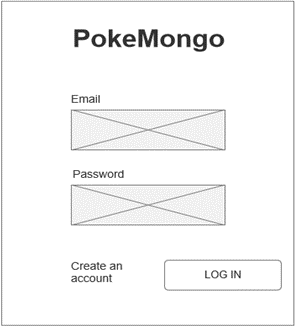
\includegraphics{img/Picture1.png}
    \caption{Login Mockup}
\end{figure}

\begin{figure}[h]
    \centering
    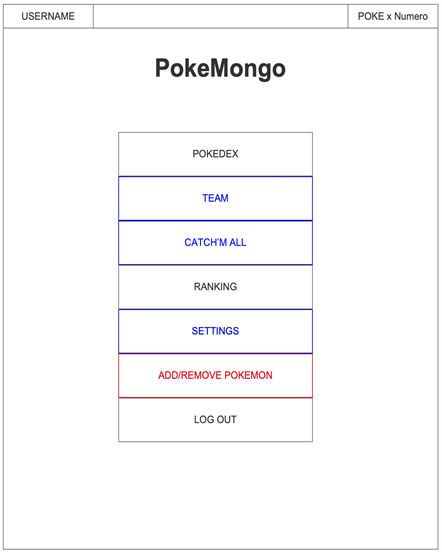
\includegraphics{img/Picture2.png}
    \caption{Homepage Mockup}
\end{figure}

\begin{figure}[h]
    \centering
    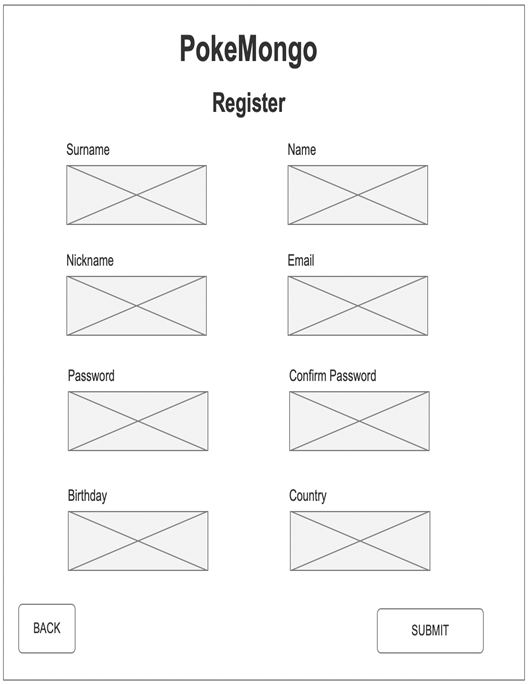
\includegraphics{img/Picture3.png}
    \caption{Signup Mockup}
\end{figure}


\begin{figure}[h]
    \centering
    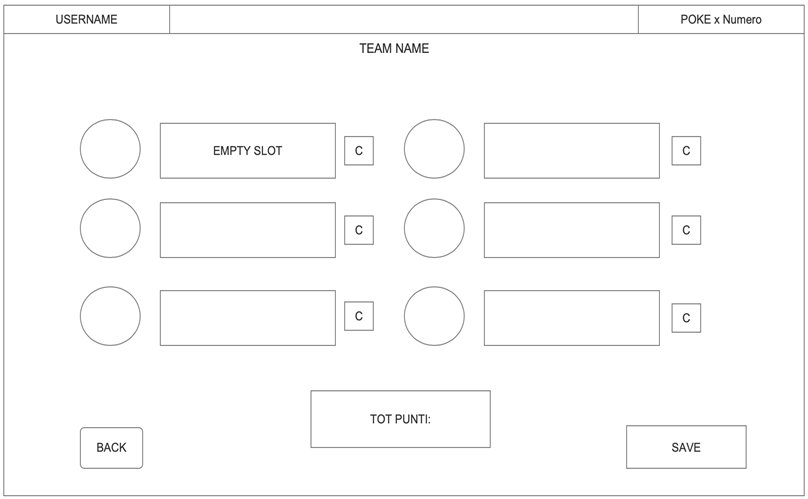
\includegraphics[width=\textwidth]{img/Picture4.png}
    \caption{Team Mockup}
\end{figure}

\begin{figure}[h]
    \centering
    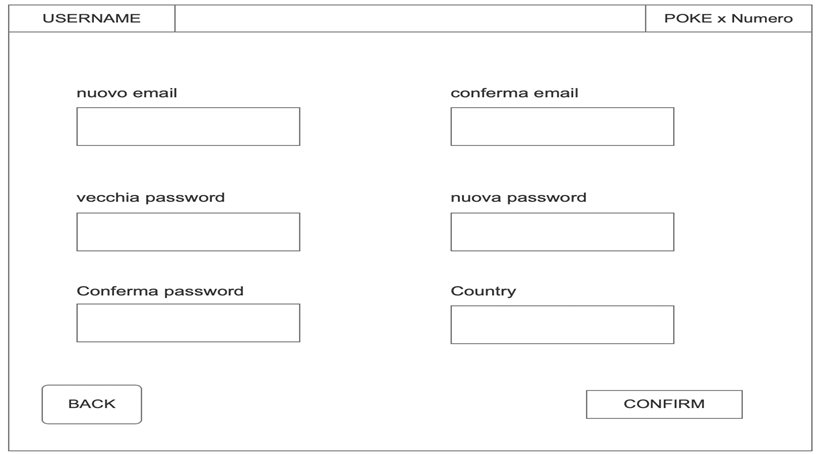
\includegraphics[width=\textwidth]{img/Picture5.png}
    \caption{Settings Mockup}
\end{figure}


\begin{figure}[h]
    \centering
    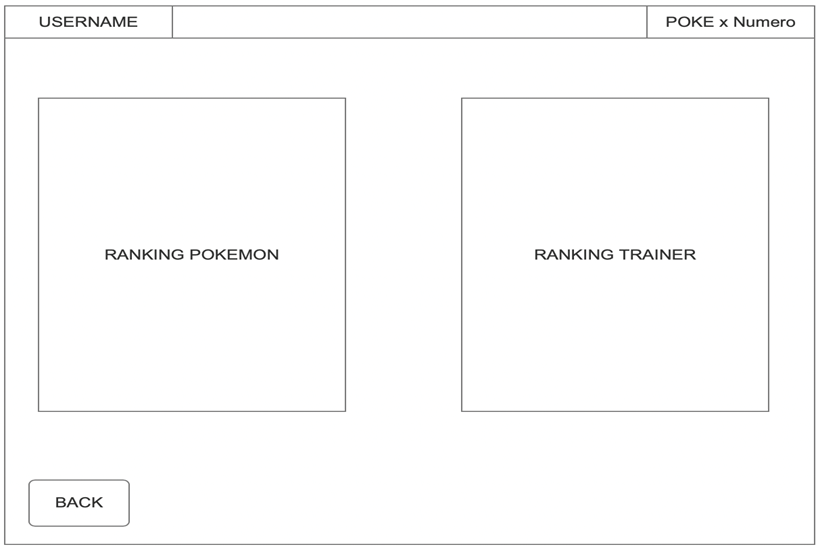
\includegraphics[width=\textwidth]{img/Picture6.png}
    \caption{Ranking Mockup}
\end{figure}
\chapter{Requirements}
\section{Something}
\begin{itemize}
    \item An \textit{unregistered user} can
    \begin{itemize}
        \item Register
    \end{itemize}
    \item A \textit{registered user} can
    \begin{itemize}
        \item Login
        \item Consult Pokèdex
        \begin{itemize}
            \item Search by name
            \item Search by type(s)
            \item Search by Pokédex ID
            \item Search by generation  
            \item Search by Pokemon characteristics (i.e, height, weight,..)	
        \end{itemize}
        \item Consult ranking:
        \begin{itemize}
            \item Most popular pokemon
            \item Best team
        \end{itemize}
        \item Team handling:
        \begin{itemize}
            \item Remove Pokemon from the team
            \item View team
            \item Save modified team
            \item View the value of the team
        \end{itemize}
        \item Catching:
        \begin{itemize}
            \item Try to catch a Pokemon to add to his team
        \end{itemize}
        \item Settings:
        \begin{itemize}
            \item Change email
            \item Change password
            \item Change country
        \end{itemize}
        \item Logout:
        \begin{itemize}
            \item Exit from the account
            \item Return to the sign in windo
        \end{itemize}
    \end{itemize}
    \item An \textit{admin} can
    \begin{itemize}
        \item Add pokemon to the Pokédex
        \item Remove pokemon from the Pokédex
    \end{itemize}
    \item The \textit{system} should
    \begin{itemize}
        \item Daily update Pokeball number of each user
    \end{itemize}
\end{itemize}
\section{Non-functional Requirements}
//To define
\section{UML relation diagram}

\begin{figure}[h]
    \centering
    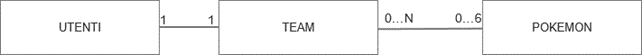
\includegraphics[width=\textwidth]{img/Picture7.png}
    \caption{Login Mockup}
\end{figure}

A user can build up only 1 team: of course, each team has just one owner.
A team is composed of a maximum of 6 Pokemons, every Pokemon can be caught by anyone, so can belong to many teams.

\include{chapters/queries_and_database_structure}


\end{document}
